\documentclass[dvipdfmx,11pt]{beamer}

%全体設定
%\AtBeginDvi{\special{pdf:tounicode 90ms-RKSJ-UCS2}}
%%%%%%%%%%%%%%%%%%%%%%%%%%%%%%%%%%%%%%%%%%%%%%%%%%%%%%%%%%%%%%%%
% User-defined Macro
%%%%%%%%%%%%%%%%%%%%%%%%%%%%%%%%%%%%%%%%%%%%%%%%%%%%%%%%%%%%%%%%
\newcommand{\compress}{\itemsep0pt\parsep0pt\parskip0pt\partopsep0pt}
% \newcommand{\compress}{\itemsep1pt plus1pt\parsep0pt\parskip0pt}
% \newcommand{\code}[1]{\lstinline[basicstyle=\ttfamily]{#1}}
\newcommand{\gringo}{\textit{gringo}}
\newcommand{\clasp}{\textit{clasp}}
\newcommand{\clingo}{\textit{clingo}}
\newcommand{\teaspoon}{\textit{teaspoon}}
\newcommand{\sat}{\textsf{SAT}}
\newcommand{\unsat}{\textsf{UNSAT}}
% \newcommand{\web}[2]{\href{#1}{#2\ \raisebox{-0.15ex}{\beamergotobutton{Web}}}}
% \newcommand{\doi}[2]{\href{#1}{#2\ \raisebox{-0.15ex}{\beamergotobutton{DOI}}}}
% \newcommand{\weblink}[1]{\web{#1}{#1}}
% \newcommand{\imp}{\mathrel{\Rightarrow}}
% \newcommand{\Iff}{\mathrel{\Leftrightarrow}}
% \newcommand{\mybox}[1]{\fbox{\rule[.2cm]{0cm}{0cm}\mbox{${#1}$}}}
% \newcommand{\mycbox}[2]{\tikz[baseline]\node[fill=#1!10,anchor=base,rounded corners=2pt] () {#2};}
% \newcommand{\naf}[1]{\ensuremath{{\sim\!\!{#1}}}}
% \newcommand{\head}[1]{\ensuremath{\mathit{head}(#1)}}
% \newcommand{\body}[1]{\ensuremath{\mathit{body}(#1)}}
% \newcommand{\atom}[1]{\ensuremath{\mathit{atom}(#1)}}
% \newcommand{\poslits}[1]{\ensuremath{{#1}^+}}
% \newcommand{\neglits}[1]{\ensuremath{{#1}^-}}
% \newcommand{\pbody}[1]{\poslits{\body{#1}}}
% \newcommand{\nbody}[1]{\neglits{\body{#1}}}
% \newcommand{\Cn}[1]{\ensuremath{\mathit{Cn}(#1)}}
% \newcommand{\reduct}[2]{\ensuremath{#1^{#2}}}
% \newcommand{\OK}{\mbox{\textcolor{green}{\Pisymbol{pzd}{52}}}}
% \newcommand{\KO}{\mbox{\textcolor{red}{\Pisymbol{pzd}{56}}}}
% \newcommand{\code}[1]{\lstinline[basicstyle=\ttfamily]{#1}}
% \newcommand{\lw}[1]{\smash{\lower2.ex\hbox{#1}}}
\newcommand{\llw}[1]{\smash{\lower3.ex\hbox{#1}}}

\newenvironment{tableC}{%
  \scriptsize
  \renewcommand{\arraystretch}{0.9}
  \tabcolsep = 0.6mm
  % \begin{tabular}[t]{p{6mm}|rlr|rlr|rlr|rlr|rlr}\hline
  %   \multicolumn{1}{l|}{\llw{問題   }} &
  \begin{tabular}[t]{l|rlr|rlr|rlr|rlr|rlr}\hline
    \multicolumn{1}{l|}{\llw{問題}} &
    \multicolumn{3}{c|}{UD1} &
    \multicolumn{3}{c|}{UD2} &
    \multicolumn{3}{c|}{UD3} &
    \multicolumn{3}{c|}{UD4} &
    \multicolumn{3}{c}{UD5} \\
    & 
    \multicolumn{1}{c}{既知の} & & \multicolumn{1}{c|}{ASP} & 
    \multicolumn{1}{c}{既知の} & & \multicolumn{1}{c|}{ASP} & 
    \multicolumn{1}{c}{既知の} & & \multicolumn{1}{c|}{ASP} & 
    \multicolumn{1}{c}{既知の} & & \multicolumn{1}{c|}{ASP} & 
    \multicolumn{1}{c}{既知の} & & \multicolumn{1}{c}{ASP} \\
    & 
    ベスト & &  & 
    ベスト & &  & 
    ベスト & &  & 
    ベスト & &  & 
    ベスト & &  \\
    \hline
  }{%
    \hline
  \end{tabular}
}


\title[ASPに基づく組合せ遷移ソルバーの実装方式に関する考察]{解集合プログラミングに基づく\\組合せ遷移ソルバーの実装方式に関する考察}
\author[山田 悠也,湊 真一,番原 睦則]{山田 悠也$^1$,湊 真一$^2$,番原 睦則$^1$}
\date{日本ソフトウェア科学会第38回大会}
\institute{1.名古屋大学 大学院情報学研究科 \\ 2.京都大学 大学院情報学研究科}

%% テンプレ 
\begin{comment}

%%%%%%%%%%%%%%%%%%%%%%%%%%%%%%%%%%%%%%%%%%%%%%%%%%
%% タイトル
%%%%%%%%%%%%%%%%%%%%%%%%%%%%%%%%%%%%%%%%%%%%%%%%%%
\begin{frame}\frametitle{}
\end{frame}

\end{comment}

%###########################################################
%# 本文 ####################################################
%###########################################################
\begin{document}

%%%%%%%%%%%%%%%%%%%%%%%%%%%%%%%%%%%%%%%%%%%%%%%%%%
%% タイトル 
%%%%%%%%%%%%%%%%%%%%%%%%%%%%%%%%%%%%%%%%%%%%%%%%%%
\begin{frame}\frametitle{}
  \titlepage
\end{frame}

%%%%%%%%%%%%%%%%%%%%%%%%%%%%%%%%%%%%%%%%%%%%%%%%%%
%% 組合せ遷移問題
%%%%%%%%%%%%%%%%%%%%%%%%%%%%%%%%%%%%%%%%%%%%%%%%%%
\begin{frame}\frametitle{組合せ遷移問題(Combinatorial Reconfiguration Problems)}

  \begin{alertblock}{}
    \alert{\bf 組合せ遷移問題}とは,
    基となる組合せ問題とその2つの実行可能解が与えられたとき,一方の実行可能解
    から他方の実行可能解へ,遷移制約を満たしつつ,
    実行可能解のみを経由して到達できるかを判定する問題.
  \end{alertblock}

  \begin{itemize}
    %\item 既存の組合せ問題の多くを組合せ遷移問題に拡張できる.
    \item 基となる問題が NP 完全であるとき,その遷移問題の多くは
      \alert{PSPACE完全}であることが知られている.
    \item 代表的な組合せ遷移問題
      \begin{itemize}
      \item 命題論理の充足可能性判定問題(SAT)の遷移問題~[Gopalan+ '09]
      \item 集合被覆問題の遷移問題~[Ito+ '11]
      \item グラフ点彩色問題の遷移問題~[Paul Bonsma+ '09]
      \end{itemize}
    \item 持続可能なシステムへの実用的応用が期待されている.
    \item 理論的な基盤が整備されつつある一方で,
          組合せ遷移問題の\alert{汎用的なソルバーの実践的な研究開発は始まったばかりである}.
  \end{itemize}
  %\begin{alertblock}{}%\centering
  %  本研究では,グラフ点彩色問題の遷移問題(\alert{$k$彩色遷移問
  %  題})をインスタンスとする.
  %\end{alertblock}
  
\end{frame}

%%%%%%%%%%%%%%%%%%%%%%%%%%%%%%%%%%%%%%%%%%%%%%%%%%
%% k彩色遷移問題
%%%%%%%%%%%%%%%%%%%%%%%%%%%%%%%%%%%%%%%%%%%%%%%%%%
\begin{frame}\frametitle{$k$彩色遷移問題}

  \begin{block}{$k$彩色遷移問題}
    \begin{itemize}
    \item 問題の入力として,グラフ点彩色問題とその二つの実行可能解
          (\structure{スタート状態}と\structure{ゴール状態})が与えられる.
    \item 遷移制約は「\structure{各遷移で色が変化する頂点はただ一つのみ}」である.
    \end{itemize}
  \end{block}

  \begin{exampleblock}{$k$彩色遷移問題の例}
    \begin{columns}
      \begin{column}{0.3\textwidth}
        \centering
        \begin{tikzpicture}
 \draw (0,0)--(8,0);
 \draw (0,1)--(8,1);
 \draw (0,2)--(8,2);
 \draw (0,3)--(8,3);
 \draw (0,4)--(8,4);
 \draw (0,5)--(8,5);
 \draw (0,6)--(8,6);
 \draw (0,7)--(8,7);
 \draw (0,8)--(8,8);
 \draw (0,0)--(0,8);
 \draw (1,0)--(1,8);
 \draw (2,0)--(2,8);
 \draw (3,0)--(3,8);
 \draw (4,0)--(4,8);
 \draw (5,0)--(5,8);
 \draw (6,0)--(6,8);
 \draw (7,0)--(7,8);
 \draw (8,0)--(8,8);
 \draw (0,0)--(0,8);
 %\fill[red] (4.5,7.5) circle (0.3);
 \draw[red] (4.5,0.5)--(4.5,7.5);
 \draw[red] (0.5,7.5)--(7.5,7.5);
 \draw[red] (0.5,3.5)--(4.5,7.5);
 \draw[red] (7.5,4.5)--(4.5,7.5);
 %\fill[cyan] (6.5,6.5) circle (0.3);
 \draw[cyan] (0.5,6.5)--(7.5,6.5);
 \draw[cyan] (6.5,0.5)--(6.5,7.5);
 \draw[cyan] (0.5,0.5)--(7.5,7.5);
 \draw[cyan] (5.5,7.5)--(7.5,5.5);
 %\fill[violet] (0.5,3.5) circle (0.3);
 \draw[violet] (0.5,3.5)--(7.5,3.5);
 \draw[violet] (0.5,0.5)--(0.5,7.5);
 \draw[violet] (0.5,3.5)--(4.5,7.5);
 \draw[violet] (0.5,3.5)--(3.5,0.5);
 %\fill[teal] (3.5,2.5) circle (0.3);
 \draw[teal] (0.5,2.5)--(7.5,2.5);
 \draw[teal] (3.5,0.5)--(3.5,7.5);
 \draw[teal] (1.5,0.5)--(7.5,6.5);
 \draw[teal] (0.5,5.5)--(5.5,0.5);
 %\fill[orange] (6.5,0.5) circle (0.3);
 \draw[orange] (0.5,0.5)--(7.5,0.5);
 \draw[orange] (6.5,0.5)--(6.5,7.5);
 \draw[orange] (6.5,0.5)--(0.5,6.5);
 \draw[orange] (6.5,0.5)--(7.5,1.5);
 \fill[red] (4.5,7.5) \symqueen ;
 \fill[cyan] (6.5,6.5) circle (0.35);
 \fill[violet] (0.5,3.5) circle (0.35);
 \fill[teal] (3.5,2.5) circle (0.35);
 \fill[orange] (6.5,0.5) circle (0.35);
\end{tikzpicture}
%        ステップ0($=\alpha$)
      \end{column}
      \begin{column}{0.05\textwidth}
        \textbf{$\longrightarrow$}
      \end{column}
      \begin{column}[]{0.3\textwidth}
        \centering
        %%%%%%%%%%%%%%%%%%%%%%%%%%%%%%%%%%%%%%%%%%%%%%%%%%
% 実行例(t=0) (第6章で使う)
%%%%%%%%%%%%%%%%%%%%%%%%%%%%%%%%%%%%%%%%%%%%%%%%%%

\begin{tikzpicture}[scale=0.6]

  % 設定
  \tikzset{node/.style={circle,draw=black}}
 
  \definecolor{col_r}{RGB}{230,0,18}
  %\definecolor{col_b}{RGB}{0,104,183}
  \definecolor{col_b}{RGB}{51,51,179}
  \definecolor{col_y}{RGB}{255,251,0}
  \definecolor{col_g}{RGB}{0,96,0}
 
  % 補助線
  % \draw [help lines,blue] (0,0) grid (20,6);
 
  % node %
  \node[node, fill=col_y!70] (node1){\textbf{1}};
  \node[node, fill=col_b!70, right=of node1] (node2){\textbf{2}};
  \node[node, fill=col_y!70, below=of node1] (node3){\textbf{3}};
  \node[node, fill=col_g!70, below=of node2] (node4){\textbf{4}};
 
  \foreach \u / \v in {node1/node2, node2/node3, node2/node4, node3/node4}
  \draw (\u) -- (\v);
 \end{tikzpicture}
 
 %%%%%%%%%%%%%%%%%%%%%%%%%%%%%%%%%%%%%%%%%%%%%%%%%%%%%%%%%%
 %%% Local Variables:
 %%% mode: japanese-latex
 %%% TeX-master: paper.tex
 %%% End:
 
%        ステップ1
      \end{column}
      \begin{column}{0.05\textwidth}
        \textbf{$\longrightarrow$}
      \end{column}
      \begin{column}{0.3\textwidth}
        \centering
        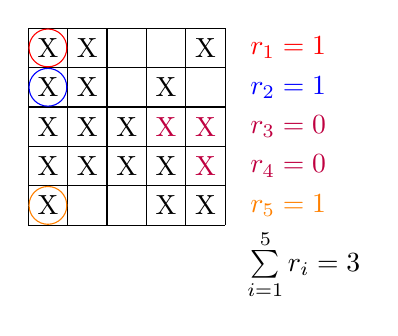
\begin{tikzpicture}
 \draw (0,0)--(2.5,0);
 \draw (0,0.5)--(2.5,0.5);
 \draw (0,1.0)--(2.5,1.0);
 \draw (0,1.5)--(2.5,1.5);
 \draw (0,2.0)--(2.5,2.0);
 \draw (0,2.5)--(2.5,2.5);
 \draw (0,0)--(0,2.5);
 \draw (0.5,0)--(0.5,2.5);
 \draw (1.0,0)--(1.0,2.5);
 \draw (1.5,0)--(1.5,2.5);
 \draw (2.0,0)--(2.0,2.5);
 \draw (2.5,0)--(2.5,2.5);
 \node (X) at (0.25,0.25) {X};
 \draw [orange] (0.25,0.25) circle[radius = 0.24];
 \node (X) at (0.25,0.75) {X};
 \node (X) at (0.25,1.25) {X};
 \node (X) at (0.25,1.75) {X};
 \draw [blue] (0.25,1.75) circle[radius = 0.24];
 \node (X) at (0.25,2.25) {X};
 \draw [red] (0.25,2.25) circle[radius = 0.24];
 \node (X) at (0.75,2.25) {X};
 \node (X) at (0.75,0.75) {X};
 \node (X) at (0.75,1.25) {X};
 \node (X) at (0.75,1.75) {X};
 \node (X) at (1.25,0.75) {X};
 \node (X) at (1.25,1.25) {X};
 \node (X) at (1.75,0.25) {X};
 \node (X) at (1.75,0.75) {X};
 \node (X) at (1.75,1.25) {\color{purple}X};
 \node (X) at (1.75,1.75) {X};
 \node (X) at (2.25,0.25) {X};
 \node (X) at (2.25,0.75) {\color{purple}X};
 \node (X) at (2.25,1.25) {\color{purple}X};
 \node (X) at (2.25,2.25) {X};
 \node (A) at (3.30,2.25) {\color{red}$r_{1} = 1$};
 \node (B) at (3.30,1.75) {\color{blue}$r_{2} = 1$};
 \node (M) at (3.30,1.25) {\color{purple}$r_{3} = 0$};
 \node (M) at (3.30,0.75) {\color{purple}$r_{4} = 0$};
 \node (C) at (3.30,0.25) {\color{orange}$r_{5} = 1$};
 \node (D) at (3.50,-0.50) {$\sum\limits_{i=1}^{5}r_{i}=3$};
\end{tikzpicture}
%        ステップ2($=\beta$)
      \end{column}
    \end{columns}
  \end{exampleblock}
  
\end{frame}

%%%%%%%%%%%%%%%%%%%%%%%%%%%%%%%%%%%%%%%%%%%%%%%%%%
%% ASP
%%%%%%%%%%%%%%%%%%%%%%%%%%%%%%%%%%%%%%%%%%%%%%%%%%
\begin{frame}\frametitle{解集合プログラミング(Answer Set Programming; ASP)}

  \begin{itemize}
    \item ASP の言語は一般拡張選言プログラムに基づく.
    \item ASPシステムは安定モデル理論~[Gelfond and Lifschitz '88] に基づく
          解集合を計算するシステムである.
    \item 近年,SAT技術の応用により高速なASPシステムが実現し, 
          システム検証やプランニングなどの様々な分野での実用的応用が拡大している.
  \end{itemize}

  \begin{alertblock}{組合せ遷移問題に対してASPを用いる利点}
    \begin{itemize}
      \item ASPの高い表現力により,記号制約を簡潔に記述できる.
      \item インクリメンタルASP解法により,同様の探索失敗を避けるために獲得した学習節を保持することで,遷移問題に対する効率的な解探索が可能である.
    \end{itemize}
  \end{alertblock}
  
\end{frame}

%%%%%%%%%%%%%%%%%%%%%%%%%%%%%%%%%%%%%%%%%%%%%%%%%%
%% ASP
%%%%%%%%%%%%%%%%%%%%%%%%%%%%%%%%%%%%%%%%%%%%%%%%%%
\begin{frame}\frametitle{ASP の基本的な構文}

  一般拡張選言プログラムのサブクラスである
  論理プログラム\footnote{標準論理プログラムを指す.}について説明する.

  \begin{itemize}
    \item \structure{論理プログラム}とは,以下の形式の
          \structure{ルール}の有限集合である.
          \begin{block}{}
            \centering
            $a_0$ \code{:-} $a_1, \dots, a_m,$ \code{not} $a_{m+1}, \dots,$ \code{not} $a_{n}$
          \end{block}
          \begin{itemize}
            \item $0 \le m \le n$であり,各$a_i$はアトム,\code{not}はデフォルトの否定,
                  ``\code{,}''は連言を表す.\code{:-}の左側をヘッド,右側をボディと呼ぶ.
            \item 直感的な意味は,「$a_1, \dots, a_m,$が成り立ち,$a_{m+1}, \dots, a_{n}$
                  が成り立たないのであれば$a_{0}$は成り立つ」である.
          \end{itemize}       
    \item ボディが空のルールを\structure{ファクト}と呼び,\code{:-}を省略できる.
          \begin{itemize}
            \item ヘッドが常に成り立つことを意味する.
          \end{itemize}
    \item ヘッドが空のルールを\structure{一貫性制約}と呼ぶ.例えば,
          \code{:-} $a_1,$ \code{not} $a_2$は,$a_1$が成り立つなら$a_2$が
          成り立つことを意味する.
  \end{itemize}
  
\end{frame}

%%%%%%%%%%%%%%%%%%%%%%%%%%%%%%%%%%%%%%%%%%%%%%%%%%
%% ASP
%%%%%%%%%%%%%%%%%%%%%%%%%%%%%%%%%%%%%%%%%%%%%%%%%%
\begin{frame}\frametitle{ASP の拡張構文}

  \begin{itemize}
    \item \structure{選択子}は
          \begin{center}
            \code{\{} $a_0$ \code{;} $\dots$ \code{;} $a_{m}$ \code{\}}
          \end{center}
          の形式で記述される.
          \begin{itemize}
            \item アトムの集合$\{ a_0, \dots, a_m\}$の任意の部分集合が成り立つことを
                  意味する.
          \end{itemize}
    \item \structure{個数制約}は
          \begin{center}
            $lb$ \code{\{} $a_0$ \code{;} $\dots$ \code{;} $a_{m}$ \code{\}} $ub$
          \end{center}
          の形式で記述される.
          \begin{itemize}
            \item $a_0, \dots, a_m$のうち,$lb$個以上$ub$個以下が成り立つことを意味する.
          \end{itemize}
  \end{itemize}
  
\end{frame}

%%%%%%%%%%%%%%%%%%%%%%%%%%%%%%%%%%%%%%%%%%%%%%%%%%
%% 研究目的
%%%%%%%%%%%%%%%%%%%%%%%%%%%%%%%%%%%%%%%%%%%%%%%%%%
\begin{frame}\frametitle{研究目的}

  \begin{alertblock}{目的}
    ASP技術を活用し,大規模な組合せ遷移問題を効率よく解くシステムを実現する.
  \end{alertblock}

  \begin{block}{研究内容}
    \begin{enumerate}
    \item 組合せ遷移問題に対して,有界組合せ遷移を提案した.
    \item 有界組合せ遷移に基づき組合せ遷移問題を解く2つのソルバーを提案した.
    \item $k$彩色遷移問題を解く2種類の符号化を提案した.
    \item 独自に作成したベンチマーク問題を用い,ソルバー及び符号化の評価実験を行った.
    \end{enumerate}
  \end{block}

\end{frame}

%%%%%%%%%%%%%%%%%%%%%%%%%%%%%%%%%%%%%%%%%%%%%%%%%%
%% 有界組合せ遷移
%%%%%%%%%%%%%%%%%%%%%%%%%%%%%%%%%%%%%%%%%%%%%%%%%%
\begin{frame}\frametitle{有界組合せ遷移}

  \begin{alertblock}{}
    \alert{\bf 有界組合せ遷移}とは,
    組合せ遷移問題に対してステップ長$\ell$を
    与え到達可能性を検査するものである.
  \end{alertblock}

  \begin{itemize}
    \item 与えられた組合せ遷移問題に対して,
          \structure{長さ$\ell$の遷移系列が存在するか}を解く.
    \item 制限された長さで系列が存在しない場合,長さを1増加させ
          再度問題を解く.
    \item 有界組合せ遷移は到達可能な遷移系列を探すのみで,
          到達不能の証明は行わない.
          \begin{itemize}
            \item ただし,適切な$\ell$の上限値を与えることで到達不能の
                  証明も行える.
          \end{itemize}
    \item 仮に遷移系列が存在する場合,得られた遷移系列は組合せ遷移問題の解の中で
          最短のものである.
  \end{itemize}

\end{frame}

%%%%%%%%%%%%%%%%%%%%%%%%%%%%%%%%%%%%%%%%%%%%%%%%%%
%% 有界組合せ遷移
%%%%%%%%%%%%%%%%%%%%%%%%%%%%%%%%%%%%%%%%%%%%%%%%%%
\begin{frame}\frametitle{有界組合せ遷移の例}

  \begin{enumerate}
    \item $\ell = 0$とする.
    \item $\ell = 0$のとき,到達不能である.
    \item $\ell = \ell + 1$とする.
    \item $\ell = 1$のとき,到達不能である.
    \item $\ell = \ell + 1$とする.
    \item $\ell = 2$のとき,到達可能である. 
  \end{enumerate}

  \begin{exampleblock}{$k$彩色遷移問題の例}
    \begin{columns}
      \begin{column}{0.3\textwidth}
        \centering
        \begin{tikzpicture}
 \draw (0,0)--(8,0);
 \draw (0,1)--(8,1);
 \draw (0,2)--(8,2);
 \draw (0,3)--(8,3);
 \draw (0,4)--(8,4);
 \draw (0,5)--(8,5);
 \draw (0,6)--(8,6);
 \draw (0,7)--(8,7);
 \draw (0,8)--(8,8);
 \draw (0,0)--(0,8);
 \draw (1,0)--(1,8);
 \draw (2,0)--(2,8);
 \draw (3,0)--(3,8);
 \draw (4,0)--(4,8);
 \draw (5,0)--(5,8);
 \draw (6,0)--(6,8);
 \draw (7,0)--(7,8);
 \draw (8,0)--(8,8);
 \draw (0,0)--(0,8);
 %\fill[red] (4.5,7.5) circle (0.3);
 \draw[red] (4.5,0.5)--(4.5,7.5);
 \draw[red] (0.5,7.5)--(7.5,7.5);
 \draw[red] (0.5,3.5)--(4.5,7.5);
 \draw[red] (7.5,4.5)--(4.5,7.5);
 %\fill[cyan] (6.5,6.5) circle (0.3);
 \draw[cyan] (0.5,6.5)--(7.5,6.5);
 \draw[cyan] (6.5,0.5)--(6.5,7.5);
 \draw[cyan] (0.5,0.5)--(7.5,7.5);
 \draw[cyan] (5.5,7.5)--(7.5,5.5);
 %\fill[violet] (0.5,3.5) circle (0.3);
 \draw[violet] (0.5,3.5)--(7.5,3.5);
 \draw[violet] (0.5,0.5)--(0.5,7.5);
 \draw[violet] (0.5,3.5)--(4.5,7.5);
 \draw[violet] (0.5,3.5)--(3.5,0.5);
 %\fill[teal] (3.5,2.5) circle (0.3);
 \draw[teal] (0.5,2.5)--(7.5,2.5);
 \draw[teal] (3.5,0.5)--(3.5,7.5);
 \draw[teal] (1.5,0.5)--(7.5,6.5);
 \draw[teal] (0.5,5.5)--(5.5,0.5);
 %\fill[orange] (6.5,0.5) circle (0.3);
 \draw[orange] (0.5,0.5)--(7.5,0.5);
 \draw[orange] (6.5,0.5)--(6.5,7.5);
 \draw[orange] (6.5,0.5)--(0.5,6.5);
 \draw[orange] (6.5,0.5)--(7.5,1.5);
 \fill[red] (4.5,7.5) \symqueen ;
 \fill[cyan] (6.5,6.5) circle (0.35);
 \fill[violet] (0.5,3.5) circle (0.35);
 \fill[teal] (3.5,2.5) circle (0.35);
 \fill[orange] (6.5,0.5) circle (0.35);
\end{tikzpicture}
        $t=0$
      \end{column}
      \begin{column}{0.05\textwidth}
        \textbf{$\longrightarrow$}
      \end{column}
      \begin{column}[]{0.3\textwidth}
        \centering
        %%%%%%%%%%%%%%%%%%%%%%%%%%%%%%%%%%%%%%%%%%%%%%%%%%
% 実行例(t=0) (第6章で使う)
%%%%%%%%%%%%%%%%%%%%%%%%%%%%%%%%%%%%%%%%%%%%%%%%%%

\begin{tikzpicture}[scale=0.6]

  % 設定
  \tikzset{node/.style={circle,draw=black}}
 
  \definecolor{col_r}{RGB}{230,0,18}
  %\definecolor{col_b}{RGB}{0,104,183}
  \definecolor{col_b}{RGB}{51,51,179}
  \definecolor{col_y}{RGB}{255,251,0}
  \definecolor{col_g}{RGB}{0,96,0}
 
  % 補助線
  % \draw [help lines,blue] (0,0) grid (20,6);
 
  % node %
  \node[node, fill=col_y!70] (node1){\textbf{1}};
  \node[node, fill=col_b!70, right=of node1] (node2){\textbf{2}};
  \node[node, fill=col_y!70, below=of node1] (node3){\textbf{3}};
  \node[node, fill=col_g!70, below=of node2] (node4){\textbf{4}};
 
  \foreach \u / \v in {node1/node2, node2/node3, node2/node4, node3/node4}
  \draw (\u) -- (\v);
 \end{tikzpicture}
 
 %%%%%%%%%%%%%%%%%%%%%%%%%%%%%%%%%%%%%%%%%%%%%%%%%%%%%%%%%%
 %%% Local Variables:
 %%% mode: japanese-latex
 %%% TeX-master: paper.tex
 %%% End:
 
        $t=1$
      \end{column}
      \begin{column}{0.05\textwidth}
        \textbf{$\longrightarrow$}
      \end{column}
      \begin{column}{0.3\textwidth}
        \centering
        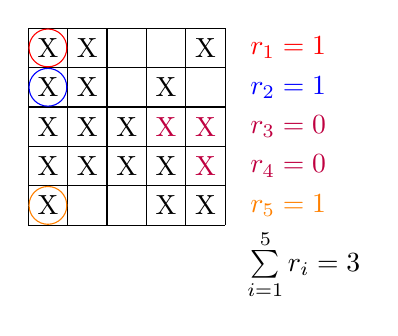
\begin{tikzpicture}
 \draw (0,0)--(2.5,0);
 \draw (0,0.5)--(2.5,0.5);
 \draw (0,1.0)--(2.5,1.0);
 \draw (0,1.5)--(2.5,1.5);
 \draw (0,2.0)--(2.5,2.0);
 \draw (0,2.5)--(2.5,2.5);
 \draw (0,0)--(0,2.5);
 \draw (0.5,0)--(0.5,2.5);
 \draw (1.0,0)--(1.0,2.5);
 \draw (1.5,0)--(1.5,2.5);
 \draw (2.0,0)--(2.0,2.5);
 \draw (2.5,0)--(2.5,2.5);
 \node (X) at (0.25,0.25) {X};
 \draw [orange] (0.25,0.25) circle[radius = 0.24];
 \node (X) at (0.25,0.75) {X};
 \node (X) at (0.25,1.25) {X};
 \node (X) at (0.25,1.75) {X};
 \draw [blue] (0.25,1.75) circle[radius = 0.24];
 \node (X) at (0.25,2.25) {X};
 \draw [red] (0.25,2.25) circle[radius = 0.24];
 \node (X) at (0.75,2.25) {X};
 \node (X) at (0.75,0.75) {X};
 \node (X) at (0.75,1.25) {X};
 \node (X) at (0.75,1.75) {X};
 \node (X) at (1.25,0.75) {X};
 \node (X) at (1.25,1.25) {X};
 \node (X) at (1.75,0.25) {X};
 \node (X) at (1.75,0.75) {X};
 \node (X) at (1.75,1.25) {\color{purple}X};
 \node (X) at (1.75,1.75) {X};
 \node (X) at (2.25,0.25) {X};
 \node (X) at (2.25,0.75) {\color{purple}X};
 \node (X) at (2.25,1.25) {\color{purple}X};
 \node (X) at (2.25,2.25) {X};
 \node (A) at (3.30,2.25) {\color{red}$r_{1} = 1$};
 \node (B) at (3.30,1.75) {\color{blue}$r_{2} = 1$};
 \node (M) at (3.30,1.25) {\color{purple}$r_{3} = 0$};
 \node (M) at (3.30,0.75) {\color{purple}$r_{4} = 0$};
 \node (C) at (3.30,0.25) {\color{orange}$r_{5} = 1$};
 \node (D) at (3.50,-0.50) {$\sum\limits_{i=1}^{5}r_{i}=3$};
\end{tikzpicture}
        $t=2$
      \end{column}
    \end{columns}
  \end{exampleblock}
  
\end{frame}

%%%%%%%%%%%%%%%%%%%%%%%%%%%%%%%%%%%%%%%%%%%%%%%%%%
%% 有界組合せ遷移
%%%%%%%%%%%%%%%%%%%%%%%%%%%%%%%%%%%%%%%%%%%%%%%%%%
\begin{frame}\frametitle{有界組合せ遷移を表す命題論理式}

  \begin{itemize}
    \item 基の組合せ問題の変数集合
          $\bm{x} = \{x_1,x_2,\ldots,x_n\}$とする.
    \item 各遷移ステップ$t\geq 0$に対して,
          ステップ$t$での各変数の値を表す変数集合
          $\bm{x}^{t} = \{x_1^t,x_2^t,\ldots,x_n^t\}$
          を導入する.
  \end{itemize}

  ステップ長$\ell$を与えたときに構成される論理式を
  $\varphi_{\ell}$とすると,
  \begin{block}{}
    \centering
    $
      \varphi_{\ell} = S(\bm{x}^0)
      \land \bigwedge_{t=0}^{\ell} C(\bm{x}^t) 
      \land \bigwedge_{t=1}^{\ell} T(\bm{x}^{t-1},\bm{x}^{t})
      \land G(\bm{x}^\ell)
    $
  \end{block}

  \begin{itemize}
    \item $S(\bm{x}^0)$はスタート状態の制約を表す論理式である.
    \item $C(\bm{x}^t)$はステップ数$t$における,
          基の組合せ問題の制約を表す論理式である.
    \item $T(\bm{x}^{t-1},\bm{x}^{t})$はステップ数$t-1$と$t$間の,
          遷移制約を表す論理式である.
    \item $G(\bm{x}^\ell)$はゴール状態の制約を表す論理式である.
  \end{itemize}

\end{frame}

%%%%%%%%%%%%%%%%%%%%%%%%%%%%%%%%%%%%%%%%%%%%%%%%%%
%% 基本ソルバー
%%%%%%%%%%%%%%%%%%%%%%%%%%%%%%%%%%%%%%%%%%%%%%%%%%
\begin{frame}\frametitle{提案する基本ソルバー}

  \begin{block}{基本ソルバーの手続き}
    \centering
    \begin{enumerate}
      \item ステップ長$\ell=0$とする.
      \item ASP システムを起動する.
      \item $\varphi_{\ell}$を論理プログラムとして記述する. \label{based_solver:loop}
      \item 論理プログラムとファクト形式の問題インスタンスを
            ASP システムに与える.
      \item ASP システムの出力が充足可能であれば終了する.
            充足不能であれば$\ell$を1増加させ,
            ASP システムを終了し,
            \ref{based_solver:loop}に戻り繰り返す.
            \begin{itemize}
              \item $\ell$が基の問題の実行可能解の総数以上になったところで
                    繰り返しを停止できる.
            \end{itemize}
    \end{enumerate}
  \end{block}

  \begin{itemize}
    \item 基本ソルバーは手続きを単純に実装したものである.
  \end{itemize}

\end{frame}

%%%%%%%%%%%%%%%%%%%%%%%%%%%%%%%%%%%%%%%%%%%%%%%%%%
%% 基本ソルバー
%%%%%%%%%%%%%%%%%%%%%%%%%%%%%%%%%%%%%%%%%%%%%%%%%%
\begin{frame}\frametitle{基本ソルバーにおける$k$彩色遷移問題の ASP 符号化}

  $k$彩色遷移問題を解く2つの ASP 符号化,
  \code{changed}と\code{unchanged}を考案した.

  \begin{exampleblock}{}\centering
    \lstinputlisting{code/gcrp_cc_changed.lp}
  \end{exampleblock}

  %\begin{block}{}\centering
  %  $k$彩色遷移問題を解く3種類のASP符号化,vrc1, vrc2, vrc3 を考案.
  %\end{block}
  %
  %\begin{itemize}
  %\item 各符号化は,
  %  \structure{「各遷移で色が変化する頂点はただ一つのみ」}という遷
  %  移制約の表現方法が異なる.
  %\item 表中の$|V|$は,グラフの頂点数を表す.
  %\end{itemize}
  %
  %\begin{exampleblock}{}\centering
  %  \begin{tabular}{l|p{8cm}}
  符号化名 & 遷移制約 \\\hline
  origin & 任意の二つの頂点に対し違反する組合せを列挙することで表現  \\ \hline
  changed & 遷移制約を ASP の個数制約を用いて表現\\\hline
  unchanged & 「各遷移で色が変化しない頂点は$|V|-1$個」という制約を,
         ASPの個数制約を用いて表現
\end{tabular}
  %\end{exampleblock}
  %
  %\begin{itemize}
  %\item 特に,vrc3符号化は基礎化後の ASP のルール数を抑えるように工夫
  %  されており,大規模な問題に対する有効性が期待できる.
  %\end{itemize}

\end{frame}

%%%%%%%%%%%%%%%%%%%%%%%%%%%%%%%%%%%%%%%%%%%%%%%%%%
%% 基本ソルバー
%%%%%%%%%%%%%%%%%%%%%%%%%%%%%%%%%%%%%%%%%%%%%%%%%%
\begin{frame}[fragile]\frametitle{ファクトと$S(\bm{x}^0)$}
  
  \begin{exampleblock}{}
    \begin{lstlisting}[]
      col(1..c).    t(0..length).
    \end{lstlisting}
  \end{exampleblock}
  \begin{itemize}
    \item 色数とステップ数をファクトで表している.
    \item \code{c}と\code{length}は定数であり,
          実行時にオプションから与えられる.
    \item \code{length}はステップ長$\ell$に対応している.
  \end{itemize}

  \begin{exampleblock}{}
    \centering
    \begin{lstlisting}
      :- not color(X,C,0), start(X,C).
    \end{lstlisting}
  \end{exampleblock}
  \begin{itemize}
    \item $S(\bm{x}^0)$に対応するルールを,
          一貫性制約を用いて表している.
  \end{itemize}

\end{frame}

%%%%%%%%%%%%%%%%%%%%%%%%%%%%%%%%%%%%%%%%%%%%%%%%%%
%% 基本ソルバー
%%%%%%%%%%%%%%%%%%%%%%%%%%%%%%%%%%%%%%%%%%%%%%%%%%
\begin{frame}[fragile]\frametitle{$C(\bm{x}^t)$}

  $C(\bm{x}^t)$は2つのルールにより表される.
  
  \begin{exampleblock}{}
    \begin{lstlisting}
      1 { color(X,C,T): col(C) } 1 :- node(X), t(T).
    \end{lstlisting}
  \end{exampleblock}
  \begin{itemize}
    \item \code{color(X,C,T)}はステップ数\code{T}において,
          頂点\code{X}が色\code{C}で塗られることを意味する.
    \item 個数制約を用いて,1つの色で塗られることを表している.
  \end{itemize}

  \begin{exampleblock}{}
    \begin{lstlisting}
      :- not { color(X,C,T); color(Y,C,T) } 1, 
         edge(X,Y), col(C), t(T).
    \end{lstlisting}
  \end{exampleblock}
  \begin{itemize}
    \item 個数制約を用いて,辺で結ばれた2つの頂点のうち,
          色\code{C}で塗られるのは1つ以下であることを表している.
          \begin{itemize}
            \item 辺で結ばれた頂点は同じ色で塗られないという制約に対応している.
          \end{itemize}
  \end{itemize}

\end{frame}

%%%%%%%%%%%%%%%%%%%%%%%%%%%%%%%%%%%%%%%%%%%%%%%%%%
%% 基本ソルバー
%%%%%%%%%%%%%%%%%%%%%%%%%%%%%%%%%%%%%%%%%%%%%%%%%%
\begin{frame}[fragile]\frametitle{$T(\bm{x}^{t-1},\bm{x}^{t})$}

  \begin{exampleblock}{}
    \begin{lstlisting}
      changed(X,T) :- color(X,C1,T), color(X,C2,T-1),
                      C1 != C2, T >= 1.
    \end{lstlisting}
  \end{exampleblock}
  \begin{itemize}
    \item ステップ数$T-1$とステップ数$T$で頂点$X$の色が変化したことを意味する
          アトム\code{changed(X,T)}を導入している.
  \end{itemize}

  \begin{exampleblock}{}
    \begin{lstlisting}
      :- not 1  { changed(X,T) } 1, t(T), T >= 1.
    \end{lstlisting}
  \end{exampleblock}
  \begin{itemize}
    \item 色が変わる頂点は各遷移において1つであることを表している.
  \end{itemize}
  \bigskip
  \begin{itemize}
    \item \code{unchanged}符号化は,$T(\bm{x}^{t-1},\bm{x}^{t})$
          の表し方が異なる.
  \end{itemize}
  
\end{frame}

%%%%%%%%%%%%%%%%%%%%%%%%%%%%%%%%%%%%%%%%%%%%%%%%%%
%% 基本ソルバー
%%%%%%%%%%%%%%%%%%%%%%%%%%%%%%%%%%%%%%%%%%%%%%%%%%
\begin{frame}[fragile]\frametitle{$G(\bm{x}^\ell)$}

  \begin{exampleblock}{}
    \begin{lstlisting}
      :- not color(X,C,length), goal(X,C).
    \end{lstlisting}
  \end{exampleblock}
  \begin{itemize}
    \item 一貫性制約を用いて表している.
  \end{itemize}
  
\end{frame}

%%%%%%%%%%%%%%%%%%%%%%%%%%%%%%%%%%%%%%%%%%%%%%%%%%
%% 基本ソルバー
%%%%%%%%%%%%%%%%%%%%%%%%%%%%%%%%%%%%%%%%%%%%%%%%%%
\begin{frame}\frametitle{基本ソルバーの問題点}

  \begin{block}{}
    \centering
    $
      \varphi_{\ell} = S(\bm{x}^0)
      \land \bigwedge_{t=0}^{\ell} C(\bm{x}^t) 
      \land \bigwedge_{t=1}^{\ell} T(\bm{x}^{t-1},\bm{x}^{t})
      \land G(\bm{x}^\ell)
    $
  \end{block}
  
  \begin{itemize}
    \item $\varphi_{\ell}$と$\varphi_{\ell-1}$に含まれる制約のほとんどは同じである.
  \end{itemize}

  \begin{block}{節集合として見たときの共通要素と非共通要素}
    \centering
    $
      \varphi_{\ell -1} \oplus \varphi_{\ell} = 
      \{C(\bm{x}^{\ell}), T(\bm{x}^{\ell -1}, 
      \bm{x}^{\ell}), G(\bm{x}^{\ell -1}), G(\bm{x}^{\ell})\}
    $ \\
    $
      \varphi_{\ell -1} \land \varphi_{\ell} =
      \{S(\bm{x}^0) \land \bigwedge_{t=0}^{\ell-1} C(\bm{x}^t)
      \land \bigwedge_{t=1}^{\ell-1} T(\bm{x}^{t-1},\bm{x}^{t})\}
    $
  \end{block}
  \bigskip

  基本ソルバーでは各$\varphi_{\ell}$に対して毎回 ASP システムを実行するため,
  \begin{itemize}
    \item 学習節が引き継がれず同一の探索空間を繰り返し調べる必要がある
    \item 同一のルールを繰り返し基礎化する必要がある
  \end{itemize}
  といった問題点が存在する.

\end{frame}

%%%%%%%%%%%%%%%%%%%%%%%%%%%%%%%%%%%%%%%%%%%%%%%%%%
%% 改良ソルバー
%%%%%%%%%%%%%%%%%%%%%%%%%%%%%%%%%%%%%%%%%%%%%%%%%%
\begin{frame}\frametitle{提案する改良ソルバー}

  \begin{block}{改良ソルバーの手続き}
    \begin{enumerate}
      \item ASP システムを起動する.
      \item ファクト形式の問題インスタンスと,
            各制約に対応したルールを表す複数のサブプログラムから構成された
            論理プログラムを与える.
      \item ステップ長$\ell=0$とする.
      \item $\ell>0$であれば,$G(\bm{x}^{\ell -1})$を
            表すルールを削除する. \label{improved_solver:loop}
      \item $\ell=0$であれば,$S(\bm{x}^0)$を
            表すルールを追加する.
      \item $C(\bm{x}^{\ell})$と$T(\bm{x}^{\ell-1},\bm{x}^{\ell})$
            を表すルールを追加する.
      \item $\varphi_{\ell}$の到達可能性を検査する.
      \item ASP システムの出力が充足可能であれば終了する.
            充足不能であれば$\ell$を1増加させ,
            ASP システムを終了し,
            \ref{improved_solver:loop}に戻り繰り返す.
            \begin{itemize}
              \item $\ell$が基の問題の実行可能解の総数以上になったところで
                    繰り返しを停止し,ASP システムを終了できる.
            \end{itemize} \label{improved_solver:end}
    \end{enumerate}
  \end{block}

  \begin{itemize}
    \item 改良ソルバーは,{\clingo}の PythonAPI を用いて実装した.
  \end{itemize}

\end{frame}

%%%%%%%%%%%%%%%%%%%%%%%%%%%%%%%%%%%%%%%%%%%%%%%%%%
%% 改良ソルバー
%%%%%%%%%%%%%%%%%%%%%%%%%%%%%%%%%%%%%%%%%%%%%%%%%%
\begin{frame}\frametitle{改良ソルバーの実装}

  続き\ref{improved_solver:loop}--\ref{improved_solver:end}
  を実装したものを以下に示す.
  \begin{exampleblock}{}
    \lstinputlisting{code/core.lp}
  \end{exampleblock}
  
\end{frame}

%%%%%%%%%%%%%%%%%%%%%%%%%%%%%%%%%%%%%%%%%%%%%%%%%%
%% 改良ソルバー
%%%%%%%%%%%%%%%%%%%%%%%%%%%%%%%%%%%%%%%%%%%%%%%%%%
\begin{frame}[fragile]\frametitle{PythonAPI (1/2)}

  \begin{itemize}
    \item 変数\code{step}はステップ長$\ell$を意味する.
  \end{itemize}

  \begin{exampleblock}{}
    \begin{lstlisting}
      parts = []
    \end{lstlisting}
  \end{exampleblock}
  \begin{itemize}
    \item ステップ長$\ell$のときに追加するルールを記憶するリストである.
  \end{itemize}

  \begin{exampleblock}{}
    \begin{lstlisting}
      parts.append(("check", [step]))
    \end{lstlisting}
  \end{exampleblock}
  \begin{itemize}
    \item 与えられる論理プログラムはいくつかのブロックに分かれている.
          ブロックはサブプログラムに相当する.
    \item \code{check}ブロックに含まれるルールに,ステップ長として$\ell=$\code{step}
          を与えたもの追加している.
  \end{itemize}

\end{frame}

%%%%%%%%%%%%%%%%%%%%%%%%%%%%%%%%%%%%%%%%%%%%%%%%%%
%% 改良ソルバー
%%%%%%%%%%%%%%%%%%%%%%%%%%%%%%%%%%%%%%%%%%%%%%%%%%
\begin{frame}[fragile]\frametitle{PythonAPI (2/2)}

  \begin{exampleblock}{}
    \begin{lstlisting}
      prg.release_external(clingo.Function
          ("query", [step-1]))
    \end{lstlisting}
  \end{exampleblock}
  \begin{itemize}
    \item $G(\bm{x}^{\ell -1})$を
          表すルールを削除している.
  \end{itemize}

  \begin{exampleblock}{}
    \begin{lstlisting}
      prg.ground(parts)
    \end{lstlisting}
  \end{exampleblock}
  \begin{itemize}
    \item 記憶したルールの基礎化を行っている.
  \end{itemize}
  
\end{frame}

%%%%%%%%%%%%%%%%%%%%%%%%%%%%%%%%%%%%%%%%%%%%%%%%%%
%% 改良ソルバー
%%%%%%%%%%%%%%%%%%%%%%%%%%%%%%%%%%%%%%%%%%%%%%%%%%
\begin{frame}\frametitle{改良ソルバーにおける ASP 符号化}

  \code{changed}符号化を改良ソルバーに対応させたものを示す.
  \begin{exampleblock}{}
    \lstinputlisting{code/gcrp_cc_changed_inc.lp}
  \end{exampleblock}
  
\end{frame}

%%%%%%%%%%%%%%%%%%%%%%%%%%%%%%%%%%%%%%%%%%%%%%%%%%
%% 改良ソルバー
%%%%%%%%%%%%%%%%%%%%%%%%%%%%%%%%%%%%%%%%%%%%%%%%%%
\begin{frame}[fragile]\frametitle{ASP 符号化の変更点 (1/2)}

  %\begin{itemize}
  %  \item ステップ数を表すファクトを削除した.
  %\end{itemize}

  \begin{exampleblock}{}
    \begin{lstlisting}
      #program base.
      #program step(t).
      #program check(t).
    \end{lstlisting}
  \end{exampleblock}
  \begin{itemize}
    \item \code{base}ブロックには,
          ファクトと制約$S$に対応するルールが含まれる.
    \item \code{step(t)}ブロックには,
          制約$C$と制約$T$に対応するルールが含まれる.
    \item \code{check(t)}ブロックには,
          制約$G$に対応するルールが含まれる.
  \end{itemize}

\end{frame}

%%%%%%%%%%%%%%%%%%%%%%%%%%%%%%%%%%%%%%%%%%%%%%%%%%
%% 改良ソルバー
%%%%%%%%%%%%%%%%%%%%%%%%%%%%%%%%%%%%%%%%%%%%%%%%%%
\begin{frame}[fragile]\frametitle{ASP 符号化の変更点 (2/2)}

  \begin{exampleblock}{}
    \begin{lstlisting}
      :- not color(X,C,t), goal(X,C), query(t).
    \end{lstlisting}
  \end{exampleblock}
  \begin{itemize}
    \item \code{query(t)}に偽を割当てることで,必ず一貫性制約を
          満たさなくなる.
    \item 一貫性制約を満たさなくすることは,
          $G(\bm{x}^{\ell -1})$を
          表すルールの削除に対応している.
  \end{itemize}
  
\end{frame}

%%%%%%%%%%%%%%%%%%%%%%%%%%%%%%%%%%%%%%%%%%%%%%%%%%
%% ベンチマーク
%%%%%%%%%%%%%%%%%%%%%%%%%%%%%%%%%%%%%%%%%%%%%%%%%%
\begin{frame}\frametitle{ベンチマークの作成}

  \begin{itemize}
    \item 組合せ遷移問題の実践的な研究は始まったばかりであり,
          ベンチマーク問題の整備も重要な課題の一つである.
    \item 本研究では$k$彩色遷移問題をベンチマーク問題として用いる.
    \item ステップ長の上限値として与える実行可能界の総数を求められる,
          グラフ点彩色問題が必要となる.
          \begin{enumerate}
            \item \textit{COLOR04}で公開されているグラフ点彩色問題のグラフ127個のうち,
                  彩色数が判明している44個~[Tamura+ '09] をベンチマーク問題の候補とした.
            \item 44個のグラフに対して,彩色数での実行可能解を全列挙することが可能
                  かを調査した.
          \end{enumerate}
    \item 総数を求められた9個のグラフから各10問ずつ,計90問のベンチマーク問題を作成した.
          \begin{itemize}
            \item スタート状態とゴール状態はランダムに選んだ.
          \end{itemize}
    \item 実行可能解の総数は,最少で120個,最大で約28億個である.
  \end{itemize}
  
\end{frame}

%%%%%%%%%%%%%%%%%%%%%%%%%%%%%%%%%%%%%%%%%%%%%%%%%%
%% 実験環境
%%%%%%%%%%%%%%%%%%%%%%%%%%%%%%%%%%%%%%%%%%%%%%%%%%

\begin{frame}\frametitle{実験概要}
  提案した2つのソルバーの評価にあたり,以下の実験を行った.
  \bigskip
  \begin{itemize}
    \item \structure{比較対象}: 
          \begin{itemize}
            \item 基本ソルバー: \code{changed}符号化と\code{unchanged}符号化
            \item 改良ソルバー: \code{changed_inc}符号化と\code{unchanged_inc}符号化
          \end{itemize}
    \item \structure{ベンチマーク問題}: 作成した$k$彩色遷移問題(90問)
    \item \structure{ステップ長の上限値}: 基となるグラフ点彩色問題の実行可能解の総数
          \begin{itemize}
            \item グラフmyciel4から作成した問題については,{\clingo}が対応している数
                  よりも解の総数が大きかったため,
                  上限値を$2^{31}-1$とした.
          \end{itemize}
    \item \structure{ASPシステム}: \textit{clingo-5.4.0} \textit{jumpy}
    \item \structure{制限時間}: 3600秒/問
    \item \structure{環境}: Mac mini,3.2GHz 6コア Intel Core i7,64GB メモリ
  \end{itemize}
  
\end{frame}

%%%%%%%%%%%%%%%%%%%%%%%%%%%%%%%%%%%%%%%%%%%%%%%%%%
%% 実験結果
%%%%%%%%%%%%%%%%%%%%%%%%%%%%%%%%%%%%%%%%%%%%%%%%%%

\begin{frame}\frametitle{実験結果: 解けた問題数}

実験結果は以下の通りである.
\bigskip

\begin{exampleblock}{}
  \centering
  \scalebox{0.8}{\begin{tabular}{l|rr|rr} 
  & \multicolumn{2}{c|}{基本ソルバー} & \multicolumn{2}{c}{改良ソルバー} \\
  & \code{changed} & \code{unchanged} & \code{changed} & \code{unchanged} \\ \hline
  解けた問題数(到達可能) & 11 & 11 & 11 & 11 \\
  解けた問題数(到達不能) & 10 & 10 & 56 & \alert{60} \\\hline
  平均 CPU 時間(秒) & 223.796 & 151.341 & 101.758 & \alert{59.095} \\
\end{tabular}}
\end{exampleblock}
  
  \begin{itemize}
    \item 90問中71問について,到達可能性を確認できた.
    \item \code{unchanged_inc}符号化は他が解いた問題をすべて解いていた.
    \item 改良ソルバーの有効性が確認できた.
  \end{itemize}

\end{frame}

%%%%%%%%%%%%%%%%%%%%%%%%%%%%%%%%%%%%%%%%%%%%%%%%%%
%% 実験結果
%%%%%%%%%%%%%%%%%%%%%%%%%%%%%%%%%%%%%%%%%%%%%%%%%%
\begin{frame}\frametitle{実験結果: カクタスプロット}

  \begin{figure}[h]
    \centering
    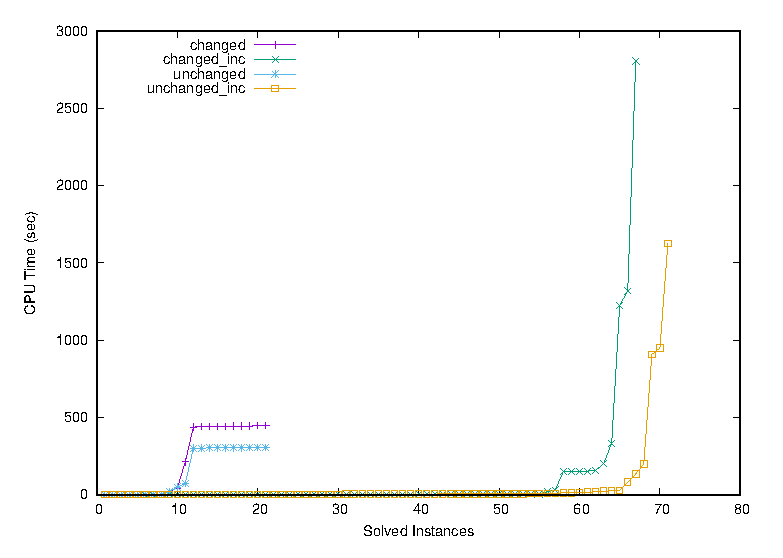
\includegraphics[scale=0.6]{fig/cactus.eps}
  \end{figure}

  \begin{itemize}
    \item 改良ソルバーは基本ソルバーより多くの問題を高速に解いている.
    \item \code{unchanged}符号化は\code{changed}符号化より多くの問題を高速に解いている.
  \end{itemize}
  
\end{frame}

%%%%%%%%%%%%%%%%%%%%%%%%%%%%%%%%%%%%%%%%%%%%%%%%%%
%% 今後の課題
%%%%%%%%%%%%%%%%%%%%%%%%%%%%%%%%%%%%%%%%%%%%%%%%%%

\begin{frame}\frametitle{まとめと今後の課題}

  \begin{block}{まとめ}
    \begin{itemize}
      \item 有界組合せ遷移を提案した.
      \item 有界組合せ遷移を解く2つのソルバーを提案した.
      \begin{itemize}
        \item 特に改良ソルバーは{\clingo}の PythonAPI を用いて高速化を図っている.
      \end{itemize}
      \item $k$彩色遷移問題を解く二つの符号化を提案した.
      \item 独自に作成したベンチマーク問題を用い,2つのソルバー及び2つの符号化の評価
            実験を行った.
      \begin{itemize}
        \item 実験の結果,改良ソルバーの優位性が確かめられた.
      \end{itemize}
    \end{itemize}
  \end{block}
  
  \begin{alertblock}{今後の課題}
    \begin{itemize}
      \item 改良ソルバーの高速化.
      \item 組合せ遷移問題の記述例の蓄積.
      \item $k$彩色遷移問題の ASP 符号化の高速化.
    \end{itemize}
  \end{alertblock}

\end{frame}

%###########################################################
%##### 補助スライド ########################################
%###########################################################

%%%% 補助スライド

\begin{frame}{~}
 \centering
 - 補足用 -
\end{frame} 

\begin{frame}{補足 : スマートグリッド}
 \begin{itemize}
  \item \structure{スマートグリッド}とは,電力の供給側,需要側において双方向の
		やり取りを可能にする次世代の\structure{賢い}電力網である.
  \item 従来と違い,通信技術の発達により,使用状況などを
		リアルタイムに把握することが可能となった.
  \item その時に応じた最適な配電網を構成し,制御するといったことが考えられている.
		\begin{itemize}
		 \item 電力需要の変化による,配電ロスの少ない構成.
		 \item 自然エネルギーによる発電量の変動を補う構成.
		\end{itemize}
  \item ASP言語の表現力や拡張性が,こうした条件の追加に活用できる可能性がある.
 \end{itemize}
\end{frame}

%%%%%%%%%%%%%%%%%%%%%%%%%%%%%%%%%%%%%%%%%%%%%%%%%%
%% 電気制約
%%%%%%%%%%%%%%%%%%%%%%%%%%%%%%%%%%%%%%%%%%%%%%%%%%
\begin{frame}{補足 : 電気制約}
 \begin{itemize}
  \item \alert{電気制約}は,送電する電流$\cdot$電圧の適正範囲を保証する制約.
  \begin{itemize}
   \item 供給経路の各区間で許容電流を超えない.
   \item 電気抵抗による電圧降下が許容範囲を超えない.
   \item etc.
  \end{itemize}
  \item 電流と電圧が影響し合う\structure{実数ドメイン上の制約}によって表される.
		% \begin{itemize}
		%  		 \item 送電システム上の条件など.
		% \end{itemize}
  \item 実数ドメイン上の制約は,純粋なASPのみで扱うのは\alert{困難}.
		\begin{itemize}
		 \item 緩和問題として,変電所から供給できる家庭の数に上限をつける.
		 \item ASPMT技術により,ASPで得られた解について,
			   背景理論ソルバーと連携して実数ドメイン上の制約を調べる.
		\end{itemize}
 \end{itemize}
\end{frame}


%%%%%%%%%%%%%%%%%%%%%%%%%%%%%%%%%%%%%%%%%%%%%%%%%%
%% 基礎化
%%%%%%%%%%%%%%%%%%%%%%%%%%%%%%%%%%%%%%%%%%%%%%%%%%
\begin{frame}{補足 : ASPシステム}
 
 \vspace{-0.5cm}

 \begin{figure}[htbp]
  \centering
  %%%%%%%%%%%%%%%%%%%%%%%%%%%%%%%%%%%%%%%%%%%%%%%%%%
%% 基礎化の流れの図
%%%%%%%%%%%%%%%%%%%%%%%%%%%%%%%%%%%%%%%%%%%%%%%%%%
\begin{tikzpicture}

 \definecolor{edge}{RGB}{38,38,134}
 \definecolor{node}{RGB}{220,220,249}

 \definecolor{alert_edge}{RGB}{191,0,0}
 \definecolor{alert_node}{RGB}{249,200,200}

 \definecolor{ex_edge}{RGB}{0,96,0}
 \definecolor{ex_node}{RGB}{230,239,230}

 \def\nodespace{2.4cm}

 \tikzset{block/.style={rectangle, thick, draw=edge, fill=node, text width=3cm, 
 text centered, rounded corners, text width=2cm, minimum height=1.5cm}};

 \tikzset{alertblock/.style={rectangle, thick, draw=alert_edge, fill=alert_node, 
 text width=3cm, text centered, rounded corners, text width=1.5cm, minimum height=1.2cm}};

 \node[block](ikkai){一階ASP\\プログラム};

 \node[rectangle,rounded corners, thick, draw=ex_edge, fill=ex_node, 
 right=0.22*\nodespace of ikkai, minimum width=6cm, minimum height=3cm, 
 text centered, label=ASPシステム](sys){};

 \node[block, right=\nodespace of ikkai](meidai){命題ASP\\プログラム};
 \node[block, right=\nodespace of meidai](ASP){解集合};

 \node[right=0.6*\nodespace of ikkai, text width=1.5cm, 
 text centered, text=red, anchor=south](){基礎化\\ソルバー};
 \node[right=0.4*\nodespace of meidai, text width=1.5cm, 
 text centered, text=red, anchor=south](){解集合\\ソルバー};

 
 \foreach \u / \v / \n in {ikkai/meidai,meidai/ASP}
 \draw [thick,->] (\u) to (\v);

\end{tikzpicture}
 \end{figure}

 \vspace{-0.5cm}

 \begin{exampleblock}{}
  \begin{enumerate}
   \item 一階ASPプログラムを基礎化ソルバーによって,
		 命題ASPプログラムに\alert{基礎化}する.
   \item 命題ASPプログラムについて,SAT技術を応用した解集合ソルバーが解集合を探索する.
  \end{enumerate}
 \end{exampleblock}

\end{frame}


%%%%%%%%%%%%%%%%%%%%%%%%%%%%%%%%%%%%%%%%%%%%%%%%%%
%% ASPのコード
%%%%%%%%%%%%%%%%%%%%%%%%%%%%%%%%%%%%%%%%%%%%%%%%%%
\begin{frame}[fragile]{補足 : 基本符号化のASPプログラム}
 \begin{exampleblock}{}
  \begin{center}
   %%%%%%%%%%%%%%%%%%%%%%%%%%%%%%%%%
   \lstinputlisting[numbers=left,%
   basicstyle=\ttfamily\tiny]{code/srf1.lp}
   %%%%%%%%%%%%%%%%%%%%%%%%%%%%%%%%% 
  \end{center}
 \end{exampleblock}
\end{frame}

\begin{frame}[fragile]{補足 : 改良符号化のASPプログラム}

 \begin{exampleblock}{}
  \begin{center}
   %%%%%%%%%%%%%%%%%%%%%%%%%%%%%%%%%
   \lstinputlisting[numbers=left,%
   basicstyle=\ttfamily\tiny]{code/srf2.lp}
   %%%%%%%%%%%%%%%%%%%%%%%%%%%%%%%%% 
  \end{center}
 \end{exampleblock}

\end{frame}



\end{document}